\section{Simulation Setup}

In order to assess the performance of the different fleet sizes and control
algorithms a novel scenario for the city of Zurich, Switzerland is set up
for the MATSim transport simulation framework. The section is structured as follows:
First, we give an overview about the used simulation components, second, we specify
the scenario and finally, we provide fleet sizing results from the theoretical
methodology presented in (cite Treleaven).

\subsection{MATSim and AMoD Simulation}

MATSim (cite Horni) is an agent-based simulation framework that makes it possible
to simulate large numbers of agents, which model a real population, in the same
traffic environment. Similar to reality, each agent has a daily plan with activities
that he wants to perform for a certain duration and finish at a specific time of
the day. Since these activities take place at different locations in the scenario,
agents need to move from activity to activity. By default, MATSim allows the
simulation of car traffic, public transit and slow modes such as going by bike
or walking. Network-based modes, such as private cars are simulated in a time-step
based manner in a network of queues with all participants at the same time. This
way it is possible that congestion emerges and agents arrive late at their
activity locations. While MATSim provides more functionality, e.g. the replanning
of agents plans to adapt to the traffic conditions that they perceive, only the
network simulation is used in this research.

An extension by Hörl (cite ABMTRANS) is used to add automated taxis to the set
of available travel modes. A virtual dispatcher, for which
different algorithms are used in this study, is constantly giving them instructions
where to go and what to do. The ``lifecycle'' of a request is always the same:
First, whenever an agents wants to depart from his current activity location by
AV, a request is issued to the dispatcher and saved. Then, an AV needs to be sent
to the customer. The choice which vehicle to send and when is completely defined
by the dispatching algorithm. Once the vehicle arrives at the customer's location
he is picked up, the AV drives to the destiation and finally drops him off. Then,
the vehicle is available for dispatching again. Alternatively, vehicles can be
rebalanced, which simply means that the dispatcher gives an AV the instruction
to drive to a different location. All of this is performed in the MATSim traffic
simulation such that AVs suffer from congestion as any other vehicle.

It should be noted that AVs drive directly to the locations where agents finish and
start their activities. So far no mechanism is implemented that would allow them
to meet at optimized locations (e.g. a high-capacity avenue instead of a small
alley).

\subsection{Scenario Definition}

For Switzerland the Microcensus on mobility and transport \cite{microcensus} is
available, which features the daily travel patterns of 60,000 Swiss residents.
It is the basis for a readily available agent population of
Switzerland, which reproduces the demographic attributes and travel patterns
in the country to great detail \cite{ivtbaseline}.

\begin{figure}[h]
\begin{center}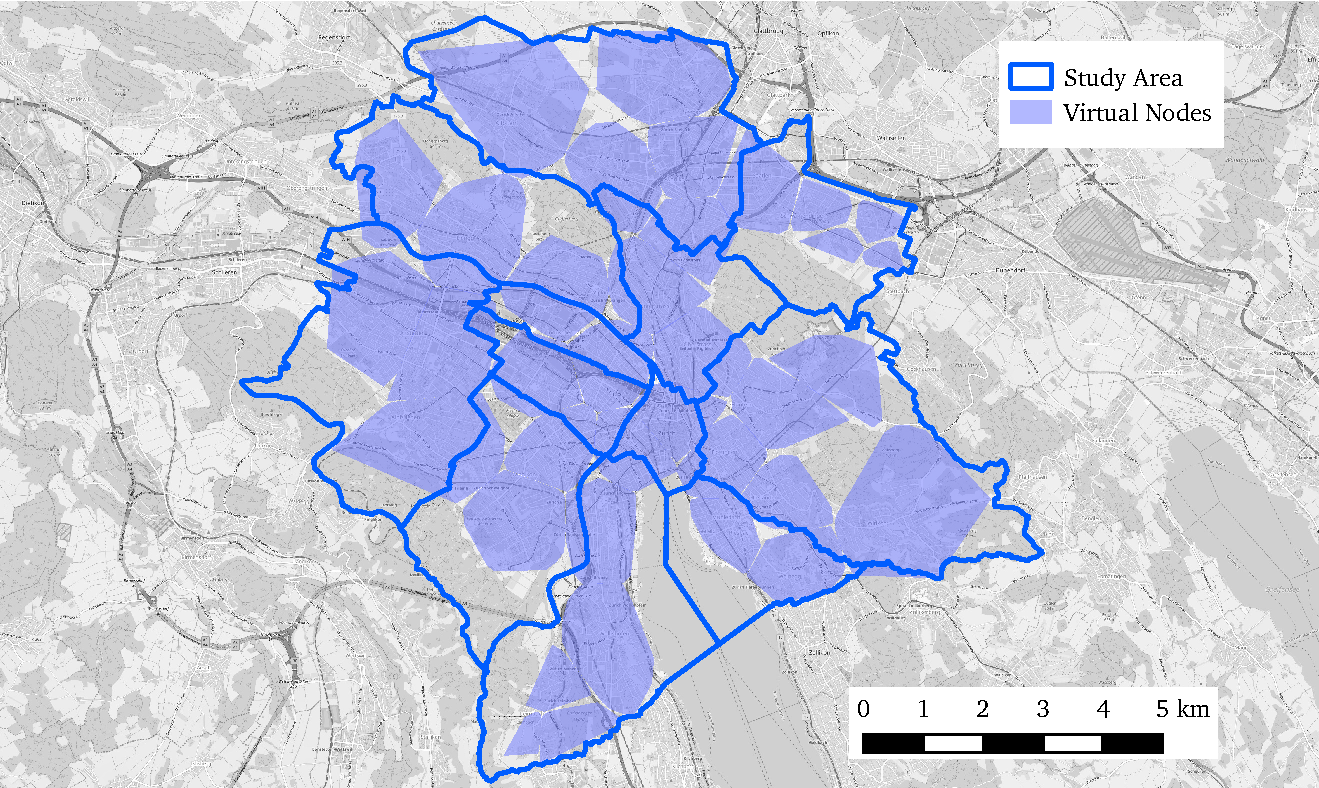
\includegraphics[width=1.0\textwidth]{figures/map.pdf}\end{center}
\caption{The study area covering the 12 districts of Zurich and the nodes of the virtual network for the rebalancing algorithms.}
\label{fig:study_area_vnodes}
\end{figure}

Additional modifications are applied to this population of around 8 million
agents to make it suitable for the study at hand. First, a best-response routing
of the travels of all agents is performed to find all agents that interfere
with the study area, which has been defined to the 12 districts of Zurich (Figure \ref{fig:study_area_vnodes}).
All agents which do not interact with that region (performing an activity within
the area or crossing the area) are deleted from the population as they do
not contribute to the state of the traffic system in that area. Finally, a 1\%
sample of the remaining agents is created, which is the basis for our
simulations. The rather extensive downscaling becomes necessary for the computationally
demanding algorithms, given that they need to be performed hundreds of times fater
than reality to allow for multiple runs and iterations.

In order to define the travel demand for the fleet of automated vehicles, agents
are tagged as whether they are viable for using an automated vehicle or not.
While pedestrians and cyclists are not simulated at all here (since they do not
contribute to congestion in the current version of the framework), agents that
travel by car or public transit at least once during their daily plan are
handled differently.

An agent that travels at least once by private car during the simulation is tagged
as an AV user \textit{only} if all of the legs in the agent's plan take place
within the study area. This constraint makes sure that no unrealistic travel
plans are generated, where an agent performs his first leg by AV although his
private car is at home and then wants to depart at the next location with that
car. Finally, the ``car'' legs of all viable agents are converted to the ``av'' mode.
All other legs are kept as before, i.e. short legs that are assigned the ``walk''
mode initially are still performed in this mode.

For agents that use public transit, the procedure is different. Here, any leg
that is performed by the ``pt'' mode in the original population is converted to ``av''
if it lies within the study area. As for car users, connecting non-motorized
legs are kept fixed.

This way a demand for Zurich is generated where each leg that possibly
\textit{can} be performed using an AV \textit{is} performed by AV. In that sense we
simulate a scenario where 100\% of the AV travel demand must be served by the
dispatchers.

To summarize, the 8,230,971 agents in the population are decimated to
1,935,400 agents, which interfere with the study area. From this set of agents
a 1\% sample has is drawn, leading to 19,354 agents that mainly constitute
background traffic for congestion. Among those are 970 agents that are viable for the AV
service. The plans of these agents contain 4030 trips that are to be served by
AVs. In reality, this service would hence need to serve 403,000 requests by
97,000 persons.

\subsection{Theoretical Fleet Sizing}

[TODO Performance driven fleet sizing for Zurich! Here EMD, minimum fleet size, fleet sizing]
